\documentclass[10pt,a4paper]{article}
\usepackage[utf8]{inputenc}
\usepackage{amsmath}
\usepackage{amsfonts}
\usepackage{amssymb}
\usepackage{graphicx}
\usepackage{float}
\usepackage[backend=bibtex]{biblatex}
\usepackage[utf8]{inputenc}
\usepackage[english]{babel}
\usepackage{graphicx}
\usepackage[a4paper, total={6in, 8in}]{geometry}
\usepackage{mathtools}
\usepackage{subfig}
\usepackage{algorithm,algpseudocode}
\usepackage{sidecap}
\usepackage{ dsfont }

 \graphicspath{{figures/}}  
\usepackage[theorems,skins]{tcolorbox}

\newtheorem{theorem}{Theorem}

\def\<{\left\langle}
\def\>{\right\rangle}
\def\vphi{\varphi}
\DeclareMathOperator{\Tr}{Tr}
\DeclareMathOperator*{\argmin}{arg\,min}
\DeclareMathOperator*{\argmax}{arg\,max}

\addbibresource{report.bib}

\begin{document}
\title{Watching CG's convergence }
\author{Marc Aurele Gilles}
\maketitle

\section{Introduction}

The convergence of Krylov subspace methods is notoriously hard to understand and reason about. For some algorithms, explicit bounds on convergence exist but are typically not informative, as the actual convergence is much faster than the one predicted by the bound. The convergence of Krylov subspace method is so unpredictable that the advice given to practitioners when they would like to know if a particular method or preconditioner would be effective for a specific problem is to try it out and see if it works. In this report we state a theorem which relates the convergence of a particular Krylov subspace method: the conjugate gradient (CG) method to the approximation of an integral through Gauss-Christoffel quadrature. 
Neither of these concepts is particularily intuitive, but the Gauss-Christoffel quadrature has a nice geometric interpretation, which allows us to visualize it. The hope is that the we can get some intuition about the convergence of CG for a specific problem by watching the associated Gauss-Christoffel quadrature problem.
The rest of the report is organized as follows: in Section \ref{sec:CG} we briefly decribe CG and some of its properties, in Section \ref{sec:quad} we define the Gauss-Christoffel quadrature and in Section \ref{sec:theorem} we link the two notions using the theorem and provide a visualization.



\section{The Conjugate Gradient Method} \label{sec:CG}

Krylov subspace methods are iterative algorithms for solving linear systems $Ax=b$. They operate by approximating the exact solution of the linear system by a sequence of the best solutions over low dimensional subspaces, called Krylov subspaces \cite{liesen_strakoss_zdenek_2013}. The $k$-th Krylov subspace of $A$ and $r_0$ is:
\begin{equation}
\mathcal{K}_k\left( A, r_0\right) = \text{span}\left\lbrace r_0, Ar_0, \dots, A^{k-1}r_0 \right\rbrace \ .
\end{equation} 
The vector $r_0$ is the initial residual $r_0 = b - Ax_0$, associated with some initial guess $x_0$.

The conjugate gradient method is a Krylov subspace method which applies when the matrix $A$ is symmetric positive definite. At the $k$-th iteration, the CG method computes the approximate solution $x_k$ that has the smallest error
\begin{equation}
e_k = x- x_k 
\end{equation}
 as measured in the $A$-norm defined by $\< x, y \>_A = \< x, Ay \>$ where $\< x,y\>$ denotes the standard Euclidean inner product over $\mathbb{R}^n$. That is, $x_k$ is uniquely defined as:
 
 \begin{equation}
 x_k = \min_{x_k\in \mathcal{K}_k(A,r_0)} \| x - x_k \|_A \ .
 \end{equation}

Some algebra on this expression leads to the 3-term recurrence which us allows to compute $x_{k+1}$ using only information from the previous two iterations. In this report we ignore many details that come into the efficient implementation of CG such as preconditioning or stopping criteria.

\subsection{Convergence Bounds}


A well-known convergence bound of the conjugate gradient method is \cite{liesen_strakoss_zdenek_2013}:
\begin{equation} \label{eq:bound}
\| e_k \|_A \leq 2 \| e_0 \|_A \left( \frac{\sqrt{\kappa(A)} -1 }{\sqrt{\kappa(A)}+1} \right)^k
 \end{equation}
where $\kappa(A) = \frac{\lambda_{\text{max}}}{\lambda_{\text{min}}}$ denotes the condition number of $A$, and $\lambda_{\text{max}}, \lambda_{\text{min}}$ denote the largest and smallest eigenvalues of $A$. Even though the CG method has the best convergence theory out of all the Krylov subspace method, it is still a rather poor one for several reasons:
\begin{enumerate}
\item It ignores the discrete nature of the spectrum of the matrix $A$. It is known that the discrete distribution of the eigenvalues of $A$ is very important to the convergence of CG.  For example, if $A \in \mathbb{R}^{n \times n}$ has only two distinct eigenvalues $\lambda_1, \lambda_2$, then its condition number can be made arbitrarily large by making the ratio $ \lambda_2 / \lambda_1$ large leading to a very weak bound, but CG will always converge in two steps.
\item The bound ignores the contribution of the right hand side. We know that the convergence of CG depends strongly on the right hand side. In particular if $b$ can be written down as a linear sum of $K$ eigenvectors of $A$, then CG provides the exact solution in at most $K$ steps.
\item It is a very poor bound. It is almost never tight in the sense that for most matrices $A$, there is no vector $b$ for which equation (\ref{eq:bound}) is equality \cite{liesen_strakoss_zdenek_2013}. Experimental results also show that the observed convergence is much faster than the one predicted by equation (\ref{eq:bound}).
\end{enumerate}

Unfortunately the convergence of Krylov subspace method is hard to think about. Better bounds than the one in equation (\ref{eq:bound}) can be derived for specific problems, but each case requires a lot of work  \cite{beckermann2001superlinear,beckermann2002superlinear}. Even if we can compute the exact solution and observe the true convergence curve, it is often difficult to understand the behavior of CG on a specific example. This motivates the theorem described in section \ref{sec:theorem}, which provides a visual way to understand the convergence of CG.

\section{Approximation of Riemann-Stieltjes Integrals} \label{sec:quad}

In this section we introduce the notion of Riemann-Stieltjes Integrals, and their approximation by quadrature. We do not give the most general definitions of the concepts, but merely the ones needed to make sense of the theorem described in section \ref{sec:theorem}.
\subsection{Riemann-Stieltjes Integrals}
Let $\omega(\lambda)$ be a non-decreasing function on $\left[ a , b \right] \subset \mathbb{R}$ with $\omega(a) =0$, $\omega(b) =1$, and  $n$ points of increase at $\{ \lambda_i \}_{i=1}^n $. That is $\omega(\lambda)$ is of the form:
\begin{equation} 
\omega(\lambda) = \begin{cases}
0 & \text{ if } a \leq \lambda \leq \lambda_1   \\
\sum_{j=1}^i \omega_j & \text{ if } \lambda_i \leq \lambda \leq \lambda_{i+1},   \quad i = 1,\dots,n-1   \\
\sum_{j=1}^n \omega_j = 1 & \text{ if } \lambda_n \leq \lambda \leq b     
\end{cases} \ .
\end{equation} 
where $\omega_j \geq 0 $. The function $\omega(\lambda)$ is often refered to as a distribution function \cite{liesen_strakoss_zdenek_2013}. Figure \ref{fig:exdist} shows an example of a distribution function.

\begin{figure}[h]
  \centering
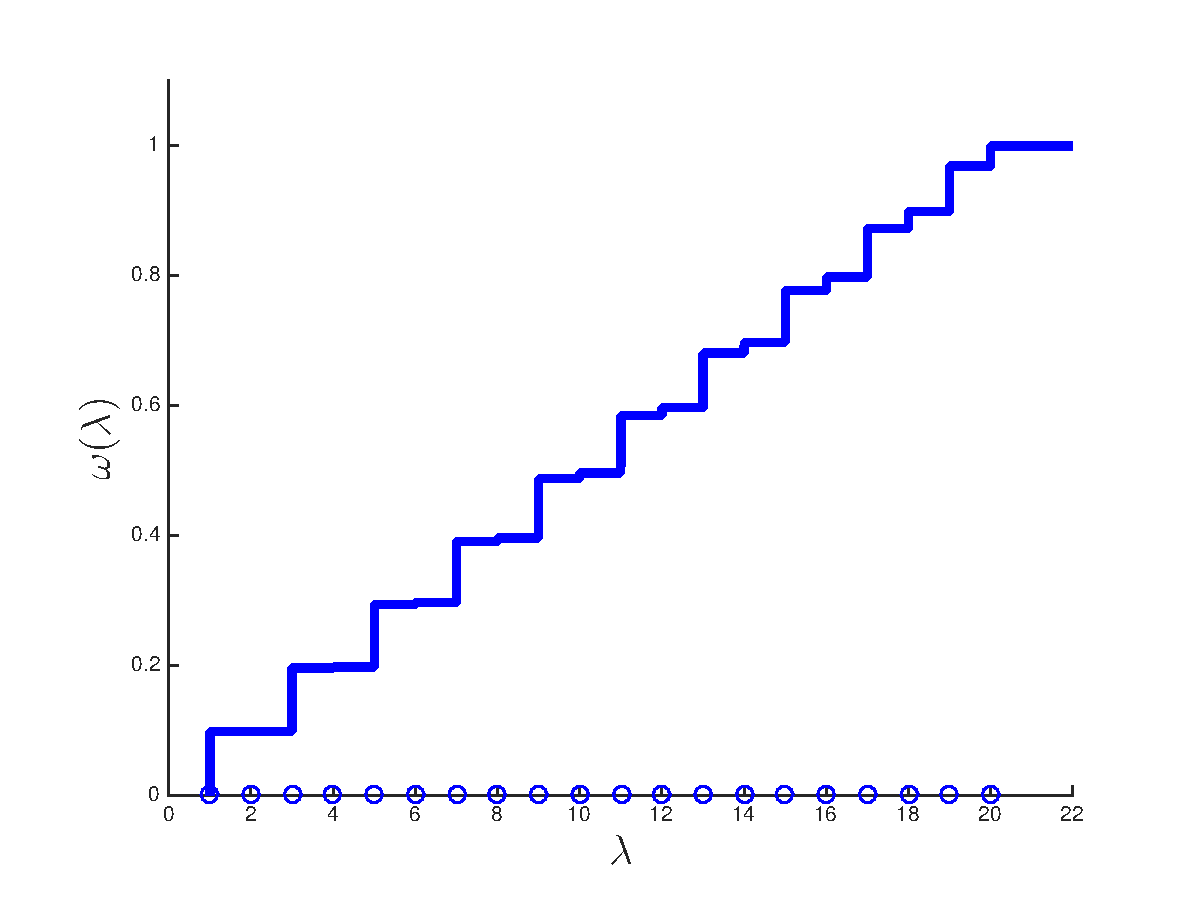
\includegraphics[width = 0.5\textwidth]{distrib}
  \caption{An example distribution function $\omega(\lambda)$  \label{fig:exdist} with points of increase at $\{ 1, 2, \dots , 20 \}$ on the interval $\left[ a , b \right] = \left[ 0, 22 \right]$ }
\end{figure}




Then for some function $f$, we can define the Riemann-Stieljes integral of $f$ with respect to $\omega$ as:
\begin{equation}
\int_a^b f(\lambda) d\omega(\lambda)  = \sum_{i=1}^n f \left( \lambda_i \right) \omega_i
\end{equation}

If $f > 0 $, the Riemann-Stieljes integral can be visualized as the area under the curve defined by $(x,y) = \left( \omega(\lambda) , f(\lambda) \right)$ for $\lambda \in \left[ a, b \right]$. Figure \ref{fig:exint} shows a visualization of the Riemann-Stieljes integral of $f(\lambda) = \frac{1}{\lambda}$ with respect to the distribution function shown in Figure \ref{fig:exdist}.

\begin{figure}[h]
  \centering
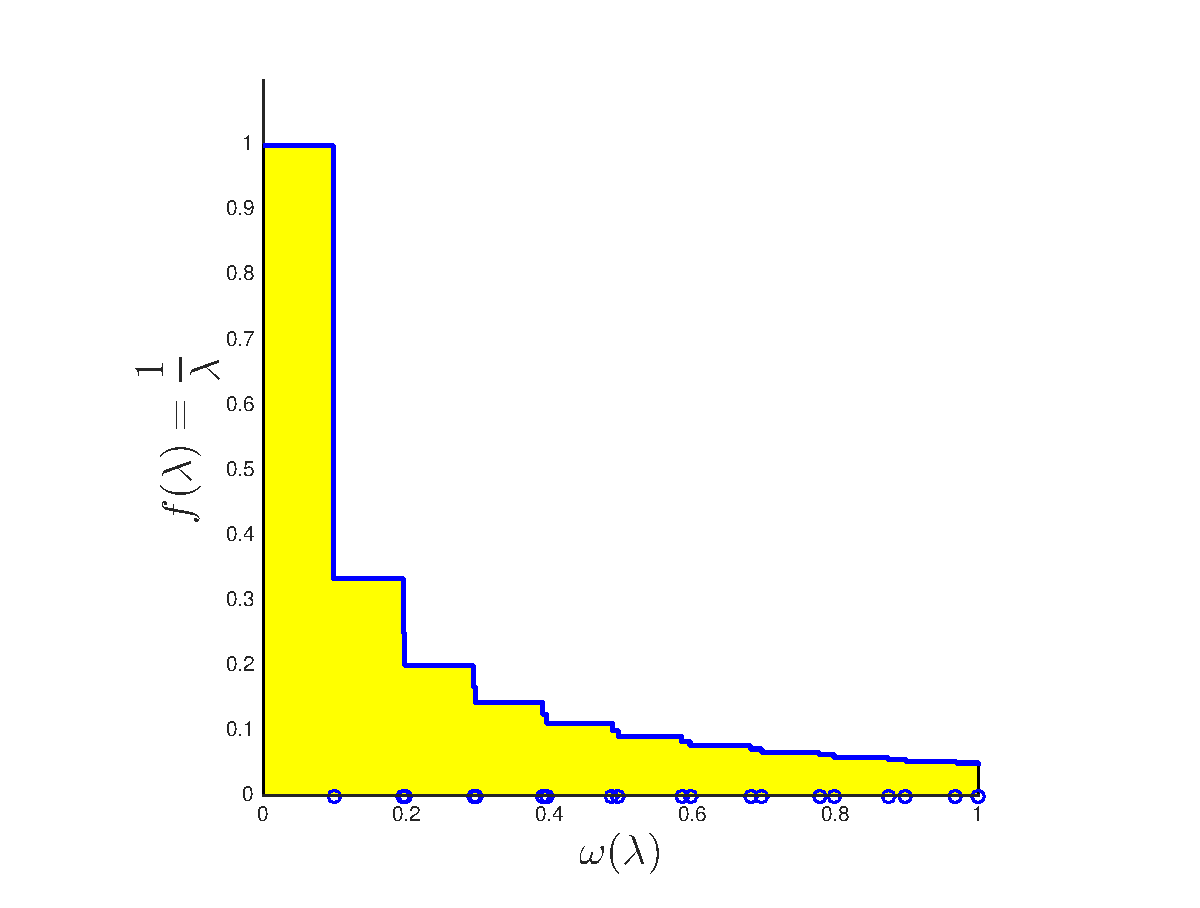
\includegraphics[width = 0.5\textwidth]{StInteg}
  \caption{Riemann–Stieltjes integral of $f(\lambda) = \frac{1}{\lambda}$ with respect to the distribution function in figure \ref{fig:exdist}. The blue curve is the curve $(x,y)=  (\omega(\lambda), f(\lambda))$, and the area of the yellow shaded region is the Riemann-Stieltjes integral. \label{fig:exint} }
\end{figure}




\subsection{Gauss-Christoffel Quadrature}

Suppose we would like to approximate the Riemann-Stieltjes integral by a weighted sum of $k$ samples of the functions. That is, for some $\theta_j^{(k)}$ (called nodes), and $w_j^{(k)}$ (called weights) , $j \in \{ 1, \dots, k \}$, we would like to approximate the Riemann Stieljes integral by:
\begin{equation}
\int_a^b f(\lambda) d\omega(\lambda) \approx \sum_{i=1}^{k} w_i^{(k)} f(\theta_i^{(k)}) \ . \nonumber
\end{equation}
We define the signed error of the approximation in the following way:
\begin{align}
E_k(f) =  \int_a^b f(\lambda) d\omega(\lambda)  -  \sum_{i=1}^{k} w_i^{(k)} f(\theta_i^k)  \nonumber \\
\iff \int_a^b f(\lambda) d\omega(\lambda)  =   \sum_{i=1}^{k} w_i^{(k)} f(\theta_i^{(k)})  + E_k(f) \nonumber \ .
\end{align}

This naturally raises the questions: where should we put the nodes (i.e. where should we sample the function)? What should the weights be?

Note that the answer is trivial if $k$, the number of nodes, is equal to $n$, the number of points of increase of $\omega$, since in that case we can set $\theta_j^{(k)}  = \lambda_j $ and $\omega_j^{(k)} = w_j$ and we have:

\begin{equation}
\int_a^b f(\lambda) d\omega(\lambda) \coloneqq \sum_{i=1}^n \omega_i f \left( \lambda_i \right) = \sum_{i=1}^{k} w_i^{(k)} f(\theta_i^k)
\end{equation}
for all functions $f$.
For other cases, one way to define a ``best" quadrature rule is to impose that the integral be exact for low degree polynomials. If this is the choice we make for optimality, then Gauss-Christoffel quadrature is a rule which provides the optimal choice. The $k$-node Gauss-Christoffel quadrature is exact for polynomials of degree $2k-1$, which can be shown to be optimal \cite{liesen_strakoss_zdenek_2013}. That is, if we pick $\theta_j^{(k)}$, $\lambda_j^{(k)}$ according to the Gauss-Christoffel quadrature rule then for all polynomials $p$ of degree at most $2k-1$:

\begin{align}
\int_a^b p(\lambda) d\omega(\lambda) = \sum_{i=1}^{k} w_i^{(k)} f(\theta_i^k) \\
\iff E_k(p) =0
\end{align}

It can be shown that the weights $w_j$ are non-negative and sum up to one, and as a consequence the nodes and weights of the $k$-node Gauss-Christoffel quadrature define a new distribution function $w^k(\lambda)$:

\begin{equation} 
w^k(\lambda) = \begin{cases}
0 & \text{ if } a \leq \lambda \leq  \theta_1^k   \\
\sum_{j=1}^i w_i^{(k)}& \text{ if }\theta_i^k\leq \lambda \leq \theta_{i+1}^k,   \quad i = 1,\dots,k-1   \\
\sum_{j=1}^n w_j^k = 1 & \text{ if } \theta_k^k \leq \lambda \leq b     
\end{cases}
\end{equation} 

The error in the Gauss-Christoffel quadrature of the function $f$, $E_k(f)$, can be visualized using this new distribution function. It is signed area between the curves defined  $(x,y) = \left( \omega(\lambda), f(\lambda) \right)$ and $(x,y) = \left( \Theta^k(\lambda), f(\lambda) \right)$. Figure \ref{fig:GaussChristEx} shows a visualization of $1$-node Gauss-Christoffel quadrature.

\begin{figure}[h]
  \centering
\includegraphics[width = 0.6\textwidth]{GaussChristEx}
  \caption{Example of $1$-node Gauss-Christoffel quadrature. Left figure: the blue plot is $\omega(\lambda)$ and the red plot is $w^{(1)}(\lambda)$. Right figure: the blue plot is the curve $(x,y) = \left( \omega(\lambda), \frac{1}{\lambda}\right) $, the red plot is $(x,y) = \left( w^{(1)}(\lambda), \frac{1}{\lambda}\right) $. The yellow and cyan regions are the regions of positive error and negative error respectively between the true integral and Gauss-Christoffel quadrature. The net error $E_1(f)$ is the area of the yellow region minus the area of the cyan region. \label{fig:GaussChristEx}}
\end{figure}




\section{Linking CG and Gauss-Christoffel Quadrature} \label{sec:theorem}

\subsection{A Special Distribution Function}
In this section we define a special distribution function in terms of a matrix $A$ and a vector $r_0$.
Let $A= \sum_{i=1}^n \lambda_i v_i v_i^T$ be an eigendecomposition of $A \in \mathbb{R}^{n \times n}$. 
We define the distribution function $\omega(\lambda)$ by setting the points of increase to $\lambda_i$, the eigenvalues of A, and setting  $\omega_i = \left( v_i^T  \frac{r_0}{\|r_0\|_2}  \right)^2$. 

For example, we take $A$ to be the finite-difference discretization of the differential operator 
\begin{equation} \label{eq:Lu}
L[u] = - \frac{ \partial^2 u }{ \partial x^2 } -  \frac{ \partial^2 u }{ \partial y^2 } + \frac{1}{2} u \quad {\text{in }} \left[ -1 , 1 \right] \times \left[ -1 , 1 \right]  
\end{equation}
 with homogenenous dirichlet boundary conditions, and $b$ to be the vector of all ones. The resulting distribution function $\omega(\lambda)$ is shown in Figure \ref{fig:Meurant}.


\subsection{Theorem by Gerard Meurant, 1997}

We are now ready to state the theorem linking the conjugate gradient method to Gauss-Christoffel quadrature:
\vfil\penalty-200\vfilneg

\begin{theorem}[G. Meurant, 1997]
The squared A-norm of the $k^{th}$ error in the CG method, scaled by the squared Euclidean norm of the initial residual, is equal to the approximation error of the $k$-node Gauss-Christoffel quadrature for $f(\lambda) = \lambda^{-1}$, with the distribution function defined by the A matrix and the normalized initial residual.
i.e.:
\begin{equation}
\int \lambda^{-1} d\omega(\lambda) = \sum_{i=1}^{k} \omega_i^{(k)} \{ \theta_i^{(k)} \}^{-1}+ \frac{\| x- x_k \|^2_A}{\| r_0 \|^2}  
\end{equation}
\end{theorem}




The theorem was proved by Gerard Meurant in 1997, but a completely equivalent statement which relates the Jacobi matrices which arise by doing Lanczos algorithm to CG was apparently already known by Stiefel, one of the inventor of the conjugate radient method \cite{golub2009matrices}. 

In this report, we view this theorem as a theoretical tool that provides a visualization, not as a useful bound for computation. Indeed, the computation of Gauss-Christoffel quadrature is much more expensive computationally than to run CG since it involves an eigenvalue computation. Nevertheless, this theorem has been used to derive estimates on the error which are computable during the iteration, and can provide good stopping criteria to the iteration. The resulting algorithm is called CGQL (conjugate gradient with quadrature and Lanczos) \cite{meurant1997computation}, and was propsed by Gerard Meurant.


Note that this theorem does not have any of the issues of the bound in equation \ref{eq:bound} that were pointed out in section \ref{sec:CG}: it takes into account the discrete distribution of eigenvalues, depends heavily on the right hand side, and is tight since the theorem is an equality.
\subsection{Visualization}

We consider the matrix $A$ defined as the finite difference approximation of  equation (\ref{eq:Lu}), the vector $b$ of all ones, and an initial guess of $x_0 =0 $ . Figure \ref{fig:Meurant} shows the visualization for this choice of $A$ and $b$.


\begin{figure}[!h]
\centering
\hspace{0in}
 \subfloat[Iteration 0 ]{
 \hspace{-2cm}
	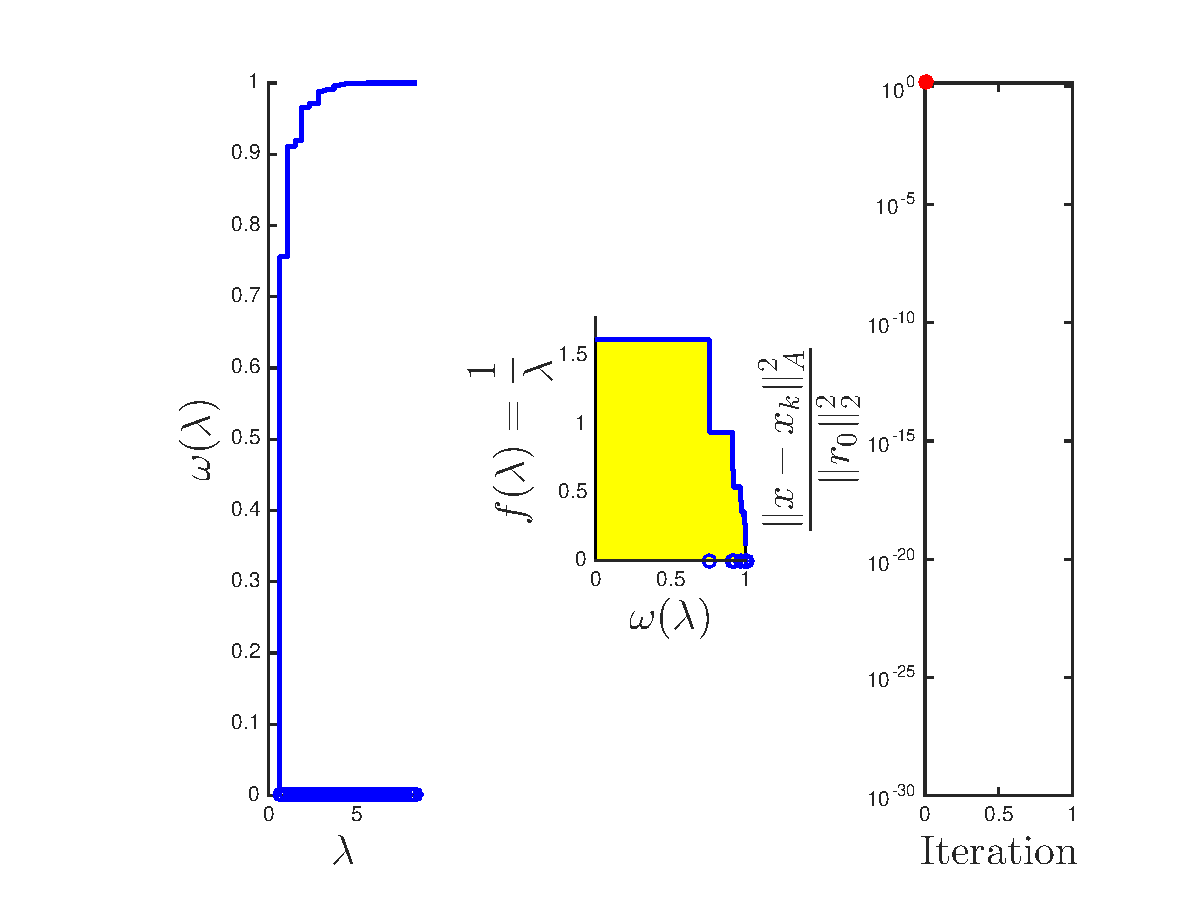
\includegraphics[width =  0.6\textwidth]{2Dpoissoniter0}
	\label{fig:subfig1}}
 \vspace{0in}
	\subfloat[Iteration 1]{
	 \hspace{-2cm}

	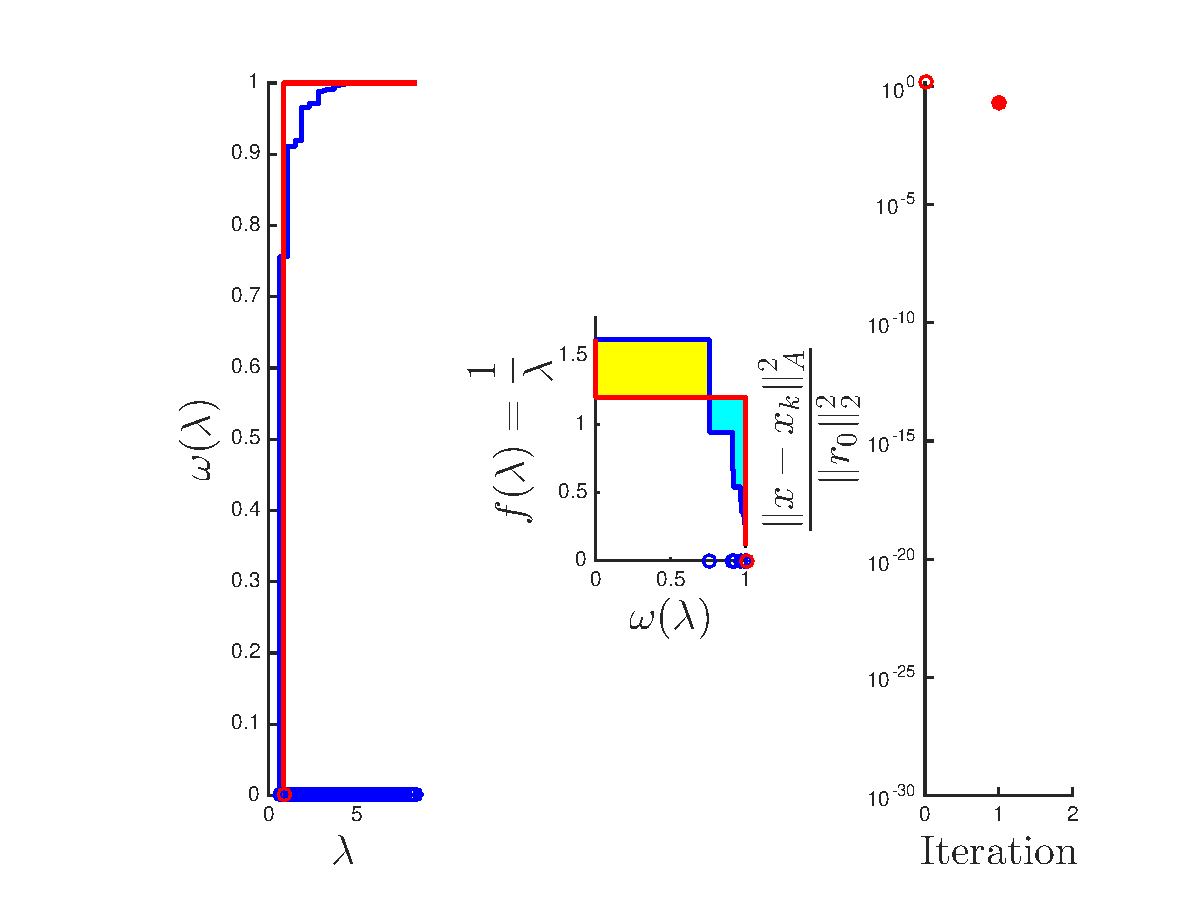
\includegraphics[width =  0.6\textwidth]{2Dpoissoniter1}
		\label{fig:subfig2}}

\hspace{0in}
 \subfloat[Iteration 3]{
 \hspace{-2cm}
	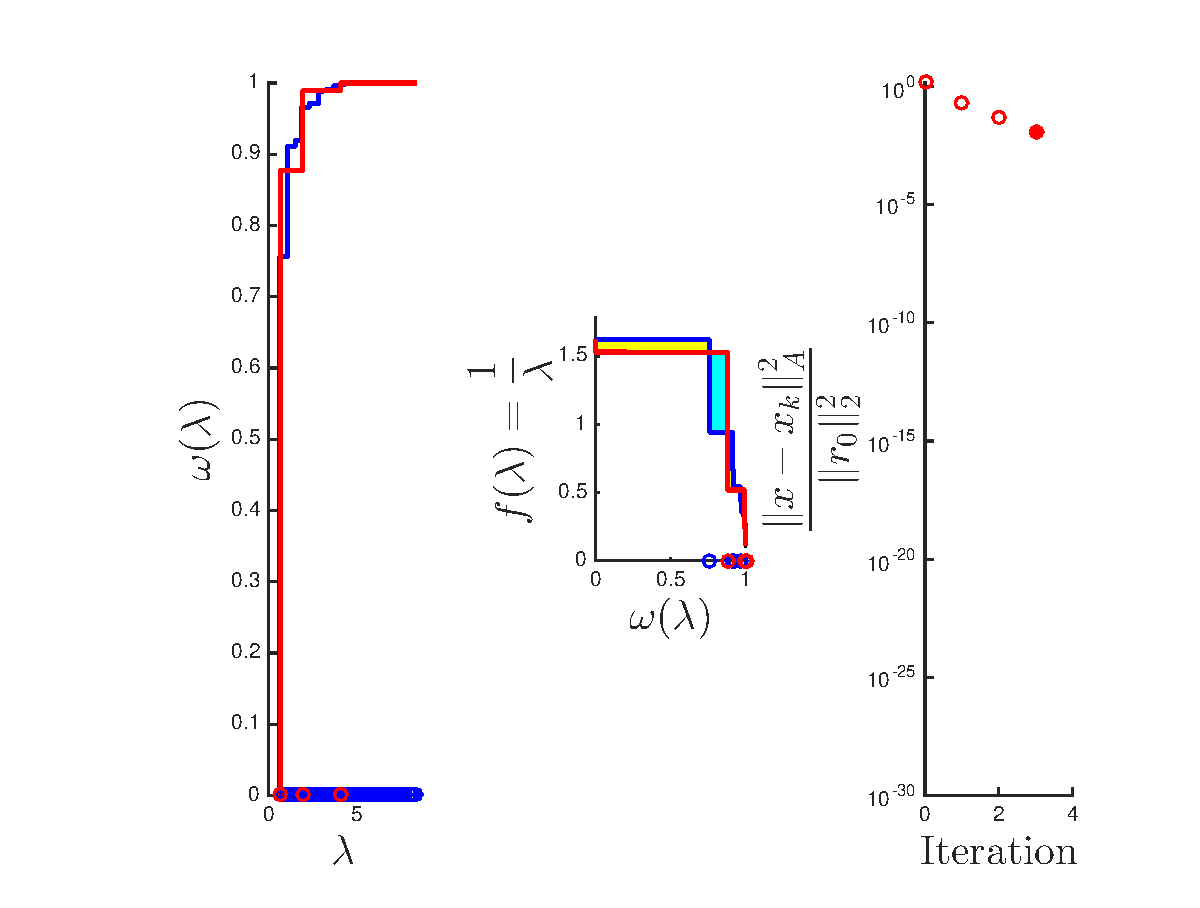
\includegraphics[width =  0.6\textwidth]{2Dpoissoniter3}
	\label{fig:subfig3}}
 \vspace{0in}
	\subfloat[Iteration 19]{
 \hspace{-2cm}
	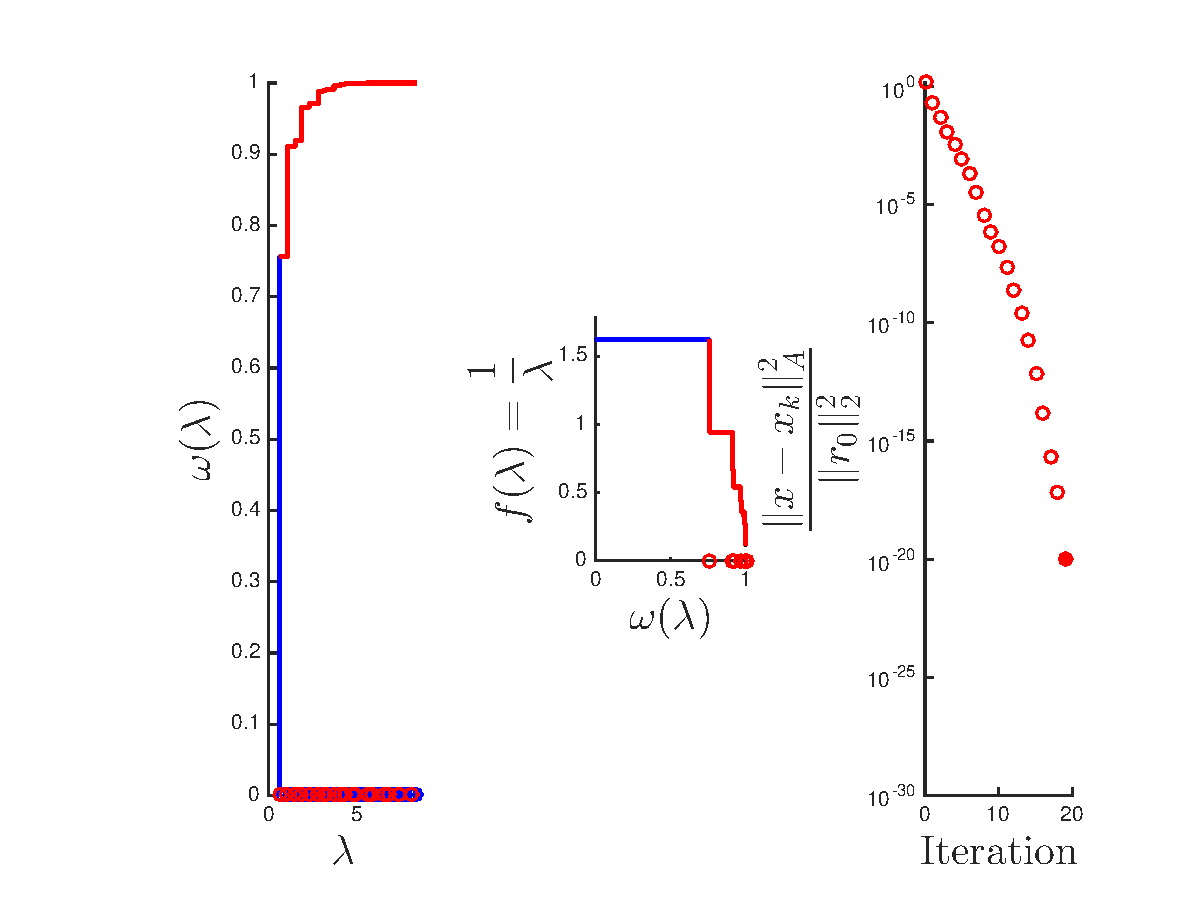
\includegraphics[width =  0.6\textwidth]{2Dpoissoniter19}
		\label{fig:subfig4}}



	  \caption{ Visualization of Meurant's theorem.  \label{fig:Meurant} }
\end{figure}

In each subfigure:
\begin{enumerate}
\item The left plot shows the distribution function $\omega(\lambda)$ in blue, the distribution function obtained  $w^{(k)}(\lambda)$ corresponding to the Gauss-Christoffel quadrature in red. The blue circles on the $x$-axis indicate the eigenvalues $\lambda_i$ of the matrix $A$, and the red circles on the $x$-axis indicate the nodes $\theta_i^{(k)}$.
\item The middle plot is a depiction of the Riemann-Stieltjes integrals of the function $f(\lambda) = \frac{1}{\lambda} $ with respect to the distribution function $\omega(\lambda)$ (area under blue curve) and $w^{(k)}(\lambda)$ (area under red curve). The positive part of the error of the Gauss-Christoffel quadrature is the area of the yellow region, and the negative part of the error is the area of the cyan region. The net signed error of the Gauss-Christoffel quadrature is the area of the yellow region minus the area of the cyan region. The blue circles on the $x$-axis indicate the eigenvalues $\omega(\lambda_i)$, the red circles on the $x$-axis indicate the points of increase of the $w^{(k)}(\theta_i^{(k)})$.
\item The right plot is the squared $A$-norm of the error at the $k$-th CG iterate, scaled by the initial residual.
\end{enumerate}
The theorem states that the net error depicted in the middle plot is equal to the value of the iterate on the right plot (depicted as the filled red dot). 

Although the visualization illustrates the theorem, it is not easy to get intuition about the convergence of CG from it. One fact that we can note for this specific problem is that the distribution function associated with the problem, has only around 15 ``visible" jumps, which is much fewer than 144, the total number of points of increase of the function, so we can expect that we only need a small number of nodes to correctly approximate the distribution function, and therefore the integral. This is confirmed by seeing that the squared error of CG at the $19$-th step is very small: around $10^{-20} $. 



\section{Conclusion}

In this report we stated a theorem which relates the error in CG to a Riemann-Stieljes integral, which can be visualized as the net area under a curve. The code for the visualization is available at https://github.com/mtg79/Meurant. It contains a few more test examples and can be run for matrix $A$ and starting residual $r_0$. For a more thorough explanation of all the concepts presented in this report, see \cite{liesen_strakoss_zdenek_2013}.

\printbibliography

\end{document}
